\section{Framework Architecture}
\label{framework:architecture}
The implemented NED Framework provides the fundamental tools and techniques on top of which a gamified system was implemented. Our ultimate goal is to demonstrate that games which are based on theoretical models and design principles can prove to be efficient in gathering qualitative annotations with minimal costs while still maintaining a large user base. Since the framework is composed of many different modules which carry various processing task and are independent from each other, an architectural model that adheres to these principles has been followed during the implementation. In other words, a micro-service architectural model has been utilized for the implementation of our framework. This section describes thoroughly all the different components composing the framework and the communication infrastructure used to exchange information between each-other. 

\subsection{The micro-service model}
%Microservice architecture
Implementing a complete monolithic architecture was seen as an unreliable and inconvenient solution for the nature of our problem. Besides the fact that many enterprises have started to shift from monolithic to micro-service architecture, considering the many benefits that the later has compared to the former, one of the reason we decided to use a micro-service architectural style is the loose-coupling of components. Ceccarelli et al. \cite{3} supports the idea that for an entity linking process a unique framework is shared where the recognition, disambiguation and linking processes are well separated and easy to isolate in order to study their performance. Therefore, a microservice architecture is best fit for our case. According to Lewis and Fowler \cite{martinfowler}, a microservice architectural style is an approach for developing a complete application as a suite of small services, which are executed individually, each on its own process and communicate with each other using lightweight mechanisms, usually over HTTP. Implementing our framework in such a way allows us to follow a more generic and abstract approach to \ac{ned} since the different modules composing the framework can be easily changed to fit for other \ac{nlp} tasks such as \ac{wsd}, co-reference resolution or even changing the language of the task to something other than English. Illustrated in Figure \ref{fig:microservice_architecture}, our framework is composed of 7 different microservices loosely coupled from each other with various responsibilities that build up the complete solution to the \ac{ned} problem.
\newpage 

\begin{figure}[]
  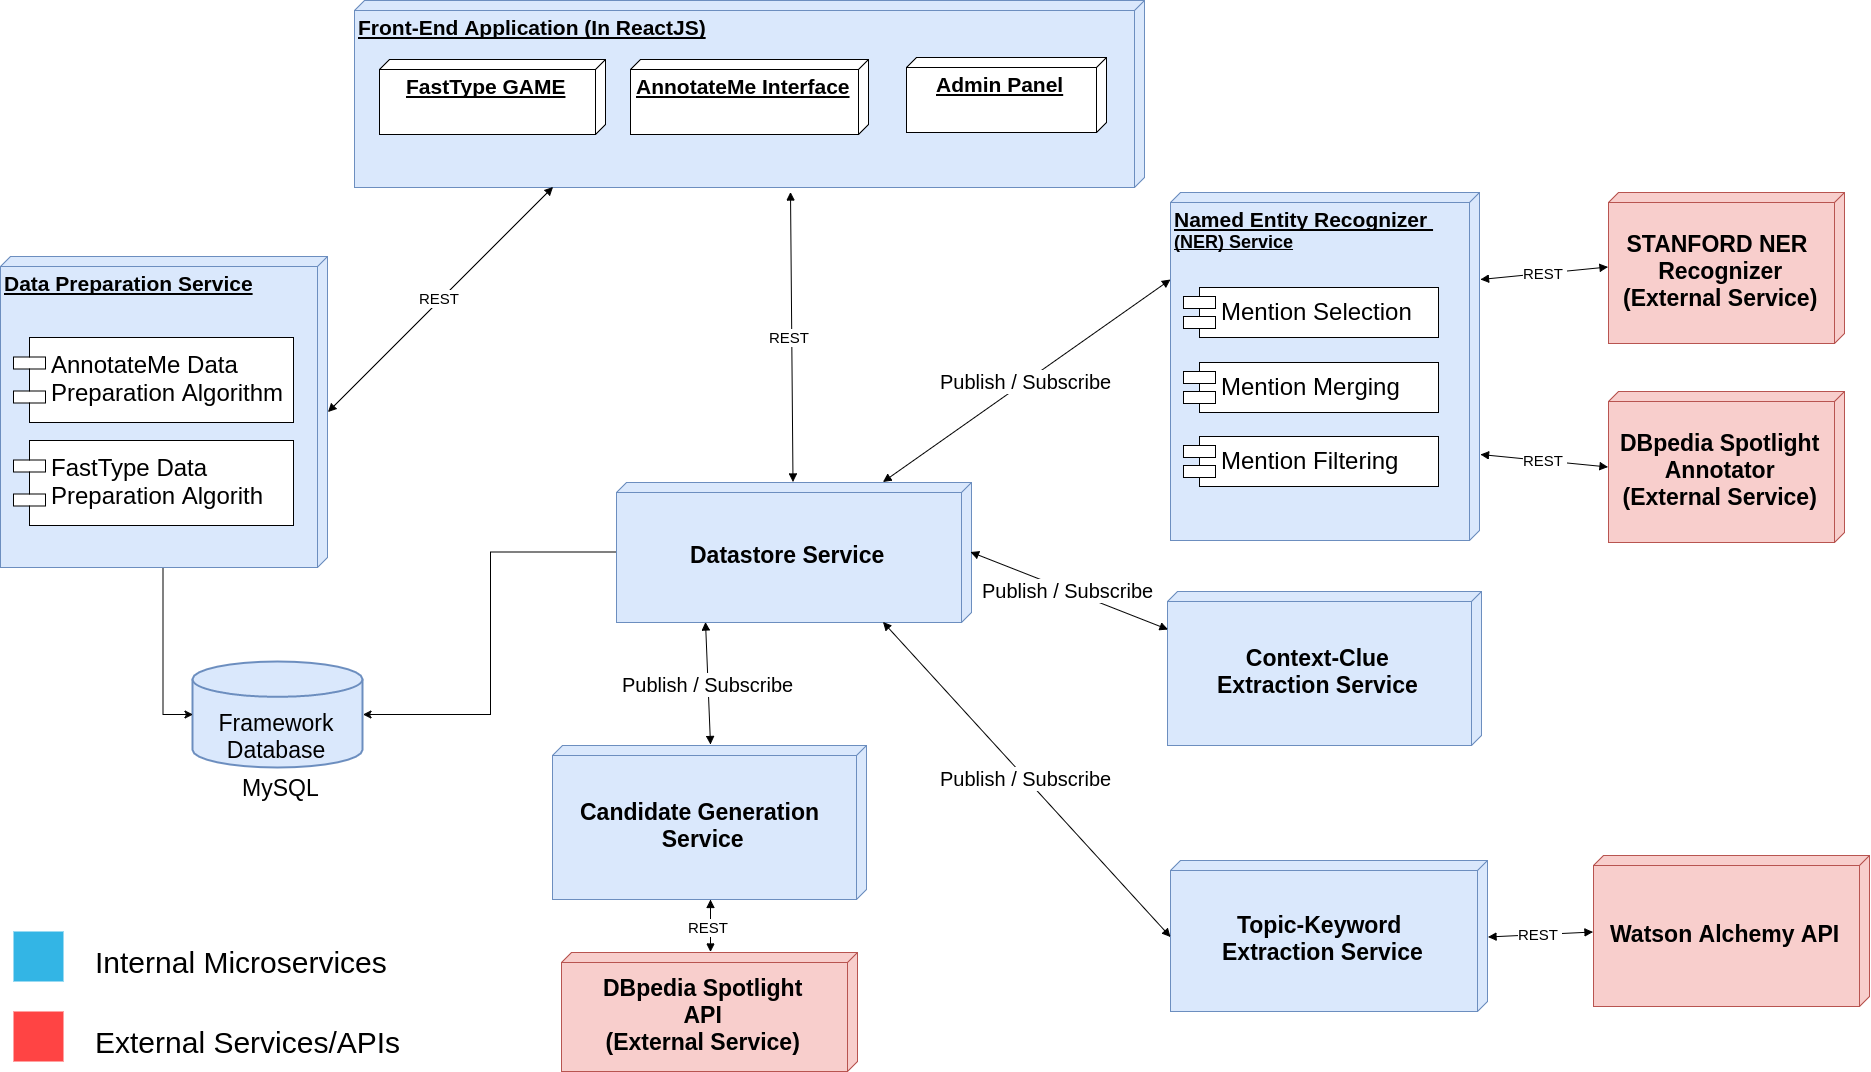
\includegraphics[width=\linewidth]{figures/microservice-architecture.png}
  \caption{Overview of the NED micro-service architecture}
  \label{fig:microservice_architecture}
\end{figure}

Observing the figure above, two different categories can be identified. The internal microservices (boxes highlighted with blue) are services that have been completely implemented from scratch. On the other hand, the external microservices (boxes highlighted in red) are external open source services that have been used by our framework to perform actions which were out of scope of this study. Among the external services, \textit{Stanford NER Recognizer} was the only external service that was not available as an online service offering API calls to perform the corresponding actions. A detailed explanation of the NER microservice is provided later in section \ref{framework:architecture_NER}.

%Communication Infrastructure
In a microservice architecture, a key factor that differs this architecture from other design patterns is the lightweight communication/messaging infrastructure. In our framework, we have utilized two different communication protocols, namely, Synchronous Messaging (\ac{rest}) and Asynchronous Messaging (\ac{amqp}). In cases where immediate response is required from a service to another, RESTful request/response API calls have been used to exchange information. We have tried to adhere to the fundamental rules of the RESTful messaging protocols where every functionality of the service is represented with a resource and operations carried out on top of these resources. As illustrated in Figure \ref{fig:microservice_architecture}, the front-end service which contains the admin panel, AnnotateMe Interface and Fastype Game communicate synchronously with the data preparation service and data store service. In addition to the front-end service, all external services are invoked using synchronous REST API calls since our internal microservices are not able to perform any internal actions unless the response from the external service is acquired. A complete documentation of the REST API calls implemented in the data store and data preparation services are available in Appendix \ref{appendix1:RESTDOCsec}.

Some of the services that compose the framework usually have a longer processing time compared to others because of the underlying complexity and the calculations that need to be performed. In these cases, it is more practical to use asynchronous messaging protocols without having to freeze the overall process as a consequence of one service which takes longer to complete. The publish and subscribe asynchronous message communication model was used for this purpose. More specifically, RabbitMQ \footnote{RabbitMQ Documentation Page \url{https://www.rabbitmq.com/documentation.html}} was used as the underlying lightweight message brooker based on \ac{amqp} (Advanced Message Queue Protocol). To see the different publishing and subscription routes that build the asynchronous communication infrastructure of the framework, see Appendix \ref{appendix1:AMQPDOCsec}.

%Conteinarization - Docker 
When designing a microservice architecture, among the many important design patterns that distinguish this architectural style from others is the deployment process. The deployment of microservices plays a critical role and when it comes to microservice architecture, the following key requirements have to be satisfied \cite{dzone}:
\begin{itemize}
    \item The ability to deploy/un-deploy independently each service
    \item It must be able to scale at each microservice level (as some services may experience more trafic than others)
    \item The ability to build and deploy microservices quickly
    \item In case one microservice fails to execute, other microservices should not be affected by this failure
\end{itemize}

To comply with the above mentioned requirements, Docker\footnote{Docker Documentation Page \url{https://docs.docker.com/}} was considered as the best microservice deployment solution. Docker is a containerization tool that lets developers and system administrators deploy self-sufficient application containers in Linux environments \cite{dzone}. Deploying a microservice into a docker container is as easy as writing a 5 line script. The steps involved to deploy an application into a docker container are as follows \cite{dzone}: 
\begin{itemize}
    \item Packaging the microservice as a Docker container image (usually by writing a script)
    \item Deploying each service instance as a container
    \item Linking containers with each other so that they are able to communicate (this is done automatically by Docker)
    \item Scaling is done by deploying many instances of the same container
    \item Building, deploying and starting a microservice is relatively fast as Docker uses containers instead of virtual machines (which is much slower compared to containers)
\end{itemize}

%Technology Stack - NodeJS, ReactJS, Mysql db
In terms of technology stack used to implement the microservice framework, the latest web technology tools have been utilized. In addition to the previously mentioned tools used for communication and deployment, the actual microservice applications framework has been implemented using NodeJS\footnote{NodeJS \url{https://nodejs.org/en/docs/}} as a back-end programming language, whereas for the front-end implementation we used ReactJS\footnote{ReactJS \url{https://facebook.github.io/react/}}. The combination of NodeJs and ReactJS has proven to be very efficient in terms of development speed, performance, agile development support and the incredible fast rendering capabilities which is very helpful during development and debugging of the application. As for the data storage, MySQL relational database has been used in our framework. 

Figure \ref{fig:workflow} illustrates the complete workflow of the framework. We use this illustration as a reference when describing the different services composing the framework in the following sections.


\begin{figure}[]
  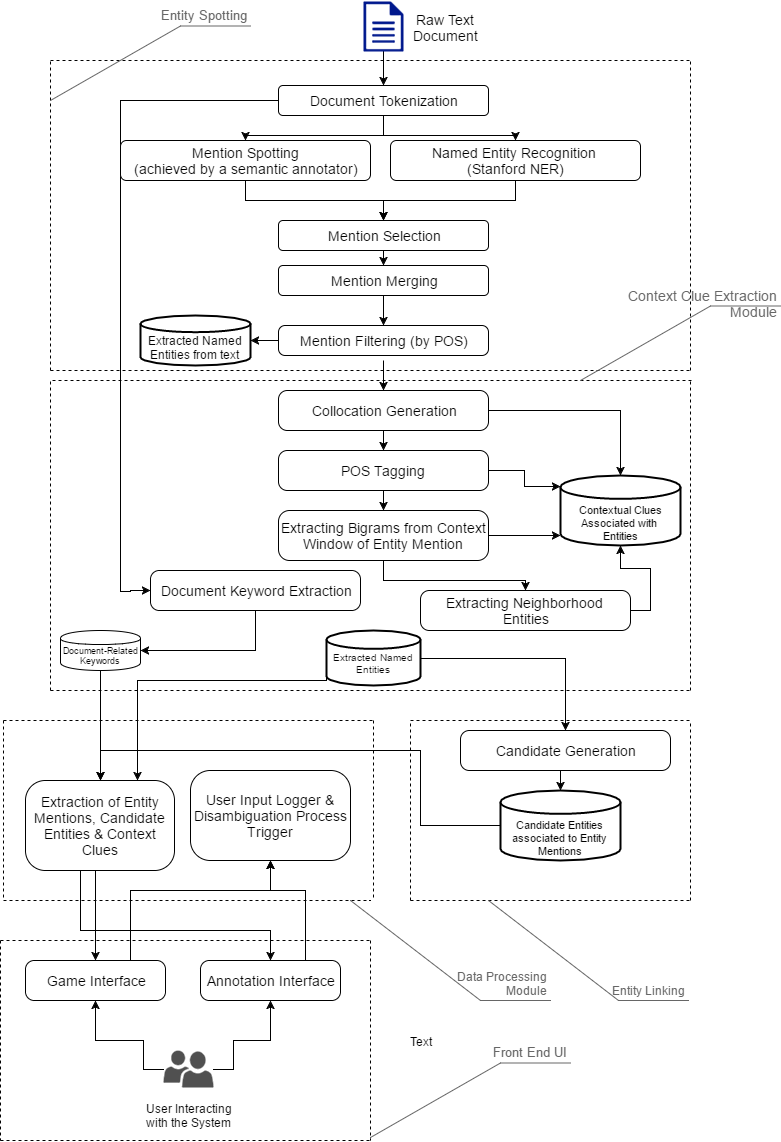
\includegraphics[width=\linewidth]{figures/workflow-diagram-v4.png}
  \caption{Overview of the complete workflow of the NED Framework}
  \label{fig:workflow}
\end{figure}


\newpage 
\subsection{Named Entity Recognition (\ac{ner}) Service}
\label{framework:architecture_NER}
The disambiguation process is initiated by uploading a raw text document through the admin panel which issues an API call to the data store service. The data store service persists the content of the document into the database and proceeds by publishing a \textit{named entity recognition} message which in turn is subscribed by the NER microservice. The published message contains all the textual content of the uploaded document. As can be seen in Figure \ref{fig:workflow}, the NER microservice starts by tokenizing the textual content of the document. A NodeJS implementation of a tokenizer has been used for this purpose \footnote{See Node Tokenizer \url{https://www.npmjs.com/package/tokenize-text}}. The tokenization process converts the text content into an array of words, sentences, characters or any other desired way. We use the tokenizer to split up sentences and individual words. 

The whole named entity recognition procedure has been inspired by \cite{39}, as they achieve very high levels of accuracy and significantly outperform state-of-the-art named entity recognizers. However, the implementation of the \ac{ner} service by Chabchoub et al. \cite{39} was carried out as part of the OKE Challenge 2016 and we were not able to find any open source code that could be integrated into our framework. Based on the information the authors provide in their publication, an attempted was made to reproduce the algorithms used in the recognition module in order to achieve similar performance levels as reported in their publication \cite{39}.

Stanford \ac{ner} \cite{standfordNER} has been used as a named entity recognizer in combination with Dbpedia Spotlight \cite{dbpedia} as a semantic annotator. Both (as external services) recognize the entities in the textual content and return a list of all the recognized entities. When comparing the results of each service, entity overlapping was observed. To be able to solve this, a selection algorithm is implemented in order to select the best entity out of both lists. The logic of the selection algorithm is keeping the longest mention and dismissing the short one. Lets take an illustrative example from the sentence below: 

\begin{quote}
\textit{"The State University of New York at Cortland celebrated its 149th anniversary this year."}
\end{quote}

In this example, Spotlight annotates \textit{State University} and \textit{New York}
 separately, whereas Stanford NER recognizes it as a single entity, namely, \textit{State University of New York}. The mention selection algorithm makes sure that the former is discarded and the later is kept. 
 
 However, even after the mention selection algorithm, it is not guaranteed that the correct entities have been identified. From the example sentence, in fact, the correct entity mention is \textit{State University of New York at Cortland}. In order to achieve this, the mention merging algorithm is performed. As explained by \cite{39}, given two named entities in close proximity, the algorithm will try to expand it to cover the next entity mention. The constraints checked by the algorithm to permit the expansion (avoiding pitfalls such as merging two legitimate different entities) have been described in detail by Chabchoub et al. \cite{39}. 
 
 The last step, before the entities are persisted into the database, consists of applying the mention filtering algorithm to the list of identified entities. The mention filtering algorithm uses a standard Part-of-Speech tagger for getting linguistic information for each entity. Accordingly, all entities that contain verbs are removed from the list, thus, filtering out incorrectly recognized entities \cite{39}. 
 
 The final result of the \ac{ner} micro-service contains a list of \textit{selected}, \textit{merged} and \textit{filtered} entities. The \ac{ner} service finalizes its process by publishing a \textit{named entity persist} message which is subscribed by the data store service that does the actual persisting of the entities into the MySQL database.

\subsection{Context Clue Extraction Services}
%Bigrams 
During the background chapter we emphasized the importance of context and how much it can affect the disambiguation accuracy for both, automatic and manual annotation systems. Referring back to the work-flow presented in the diagram in Figure \ref{fig:workflow}, contextual clues are extracted by following a three step process.

The process starts by removing all stop words in the sentences where the entity mentions are part of. After the stop words have been removed from the sentences, the \textit{collocation generation algorithm} is performed on those sentences. Collocations, according to Colson et al. \cite{52} represent the occurrence of two or more words within a short proximity between each other in text. They also argues that collocations are more likely to occur as fixed expressions such as compound nouns, proper nouns, idioms, noun-adjective combination, adjective-noun combination, verb-noun, well known song or film titles. The collocation generation algorithm follows these principles when deciding to keep a collocation from the sentence or not. Since we are dealing with analysis of grammatical structures in the sentence, part-of-speech tagging is a crucial step to be performed at this stage. 

After having extracted all potential collocations from the sentence provided as input data to the service, the next step is to associate these collocations as contextual clues to each and every entity. However, not every identified collocation within the sentence can be a useful context clue for the entity that is also part of that sentence. Previous studies have used a context window size of 4, which means that they take four preceding and four subsequent words from the sentence where the target entity occurs \cite{35}. The number 4 has been chosen because the accuracy of sense resolution does not improve when more than 4 words around the target word are considered. However, recent studies argue that the context windows size around the ambiguous target entity is dependent on the nature of the word itself \cite{35}. Our solution to this problem is increasing the context window size depending on how ambiguous the target word is. The ambiguity of a target entity is defined by the number of potential candidates extracted from the \ac{kb}. The more candidates are generated for the target entity, the higher the level of ambiguity. We believe that this represents an accurate metric on deciding the context size of the target entity. 

Since collocations can be a combination of more than two words, we have decided to keep only collocations that are composed of two words (i.e. bigrams). This decision is influenced on the findings acquired by Mihalcea and Rada \cite{36}. They observed that in terms of words in context, bigrams seem to be more effective than simple keywords and other combinations larger than two.In addition to the collocations which are considered as clues to help summarize the context in which the target word occurs, neighbour entities also also fall into this category. Since the algorithm has information on the exact position of each entity in the sentence (by maintaining a starting and ending index), we are able to decide which (other) entities are in close proximity to the target entity. Usually all identified entities that are part of the same sentence as the target entity are considered as neighbor entities. In some cases, when the sentence is short, the algorithm looks for neighbor entities in the preceding and subsequent sentences. The algorithm maintains a constraint on which it bases its logic whether to consider keeping or discarding a neighbor entity for the target entity. The constraint is basically a calculated word distance between the target entity and all other potential neighbor entities. 

After the local contextual clues have been extracted by our internal microservice, the last step is the extraction of document keywords. Document keywords are used to represent the theme or topic of the document, and might help in the disambiguation process in addition to local contextual clues. In this stage, Alchemy API is queried which extracts the most important keywords from a document. These keywords are associated as context clues to all identified entities in the same document whereas local context clues are distinct from one entity to another. Figure \ref{fig:context-clue} illustrates an example of a paragraph and the corresponding results after running the context clue extraction service. In this example, the target entity for which the context clues are to be associated is highlighted in red. The legend illustrated as a table in the example figure explains the meaning of the different colors. In cases where the words are underlined and highlighted with different colors, it means that the word combination has multiple purposes. For example "New York" from the illustrative paragraph in Figure \ref{fig:context-clue} is considered a neighbor entity to G1 (the target entity) in addition to being a keyword that contributes to understanding the meaning of the complete paragraph.


\begin{figure}[]
  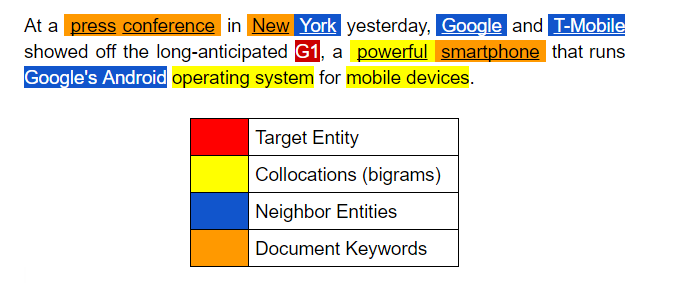
\includegraphics[width=\linewidth]{figures/context-clues.png}
  \caption{An example of a paragraph and the different contextual clues extracted from the service}
  \label{fig:context-clue}
\end{figure}

\subsection{Candidate Generation Service}
Dbpedia Spotlight is the semantic annotator which is queried by the \textit{Candidate Generation Service} to extract DBpedia candidates for a specific entity mention. No special logic has been applied in this service and therefore, the results retrieved after querying Dbpedia Spotlight are persisted into our system without additional modifications to the original data.

Dbpedia Spotlight \cite{dbpedia} performs the disambiguation process by pre-ranking entity candidates for each surface form spotted in the text. A combination of a prior score and a contextual score is calculated in order to determine which candidate entity is the most relevant. The prior score represents an estimation of how often the surface form is used as an anchor in a Wikipedia hyperlink that points to the entity page \cite{39}. Whereas the context score makes use of the context of the phrase (usually a window of words around the phrase) and the context of each candidate entity (calculated internally by Spotlight). When querying highly ambiguous entities such as "Paris" which can have over ten target candidates, only the best 8 are fetched to be evaluated. According to a user study conducted by Bontcheva et al. \cite{33}, participants gave feedback that having more than 8 options to choose from is associated with high cognitive load which results in immediately exhausting users. In addition to the maximum number of 8 candidate entities, we provide a last option called "none of them" in case the Spotlight was not able to fetch the correct candidate in the list.

During the experimental user study we observed that Spotlight was not able to provide the correct candidate entity for many entity mentions. Therefore we experimented with providing different context window sizes to the annotator to see if the performance changes. First we queried Spotlight by providing only the entity itself without any other contextual information. Second, the contextual clues extracted by our microservice were put in a sentence together with the target entity with clues located prior and after the target entity (based on where the clues were located on the original sentence). Finally, the original sentence where the target entity is part of, was used as context and sent as query parameter to Spotlight. We report in the results section of this chapter that the differences in performance between the three groups is relatively small and does not assure statistical significance.

\subsection{Data store \& data preparation service}
To assure the control and consistency of data being processed by the different microservices composing the framework, the \textit{Data-Store Service} was designed to be the only entry point to which the data could be manipulated. The service provides endpoints for accessing and manipulating the information residing on the database as a means of API calls and asynchronous message inquiries. It also serves as an information provider to the admin panel in the front-end application and also subscribes to different message routes such as: persisting named entities recognized from \ac{ner} microservice, persisting context clues and associating the generated candidate list to all registered entity mentions in the database. Besides subscribing to these message routes, the \textit{Data-Store Service} is the service endpoint that manages the complete asynchronous messaging infrastructure.

On the other hand, the \textit{Data-Preparation Service}, as the name implies, prepares the data for the AnnotateMe Interface as well as for the Fastype Game. Similar to the Data-Store Service, it has direct access to the database information with only one specific permission: reading (i.e. querying and retrieving information from the database). Therefore, for the sake of centralization and control of data, the Data-Preparation Service is considered as a read-only service with regards to the database access.

A unique feature implemented in the data preparation service is, as we like to call it, the \textit{disambiguation trigger}. This feature is responsible for resolving a specific entity mention (deciding which candidate represents the correct link for the target entity) when enough annotation data from the human annotators are accumulated. Since the most usual use-case scenario includes non-expert human annotators performing the validation process by either using the AnnotateMe Interface or the Fastype game, assuring quality of annotations is reached through redundancy. The level of redundancy maintained in the data preparation service is based on constraints proposed by Snow et al. \cite{32}. They conducted an experiment where they evaluated the quality of non-expert annotators in comparison with expert annotators. Their results indicate that on average it requires 4 independent non-expert annotations to achieve the equivalent ITA of a single expert annotator. Therefore, the disambiguation trigger is triggered when 4 independent annotations (having the same candidate as the selected option) have been accumulated for a specific entity mention. After an entity has been resolved, it will no longer show up on the interface for validation. The resolving step is done by the \textit{Data-Preparation Service} which initiates a REST API call to the \textit{Data-Store Service} in order to update the information on the databse.

%Order effects
A final element that is taken care by the \textit{Data-Preparation Service} is the ordering of candidates presented to human annotators. In a study conducted by Duarte et al. \cite{34}, they argue that in search engines, web users expect the best answer to be in the first or second position. This type of expectation represents potential bias on the results assessing the behaviour of annotators. After performing some user studies, they conclude that search result selection behaviour is influenced by ranking, with users showing tendency to select higher ranks without exploring other alternatives. To avoid having this situation in our experiment, we encourage users to explore all the candidates presented to them before making a decision. The encouragement is done by providing short descriptions for each candidate on the interface. Additionally, we avoid the chance of making users form assumptions about potential candidates being ranked higher in a list by completely randomizing the process of candidate positioning. Random positioning of alternatives instead of ranking has proven to be much more effective in encouraging users to explore all available alternatives instead of making blind decisions \cite{34}.


\newpage
\subsection{AnnotateMe Interface}

\begin{figure}[]
  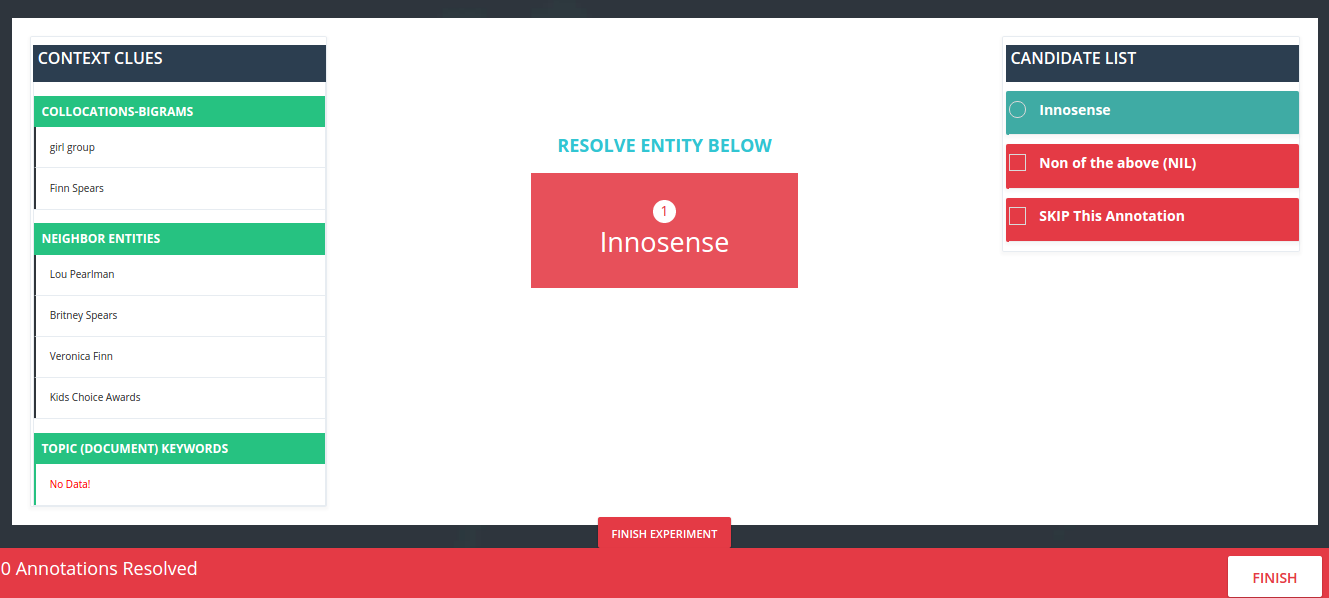
\includegraphics[width=\linewidth]{figures/annotateme-interface.png}
  \caption{The AnnotateMe Interface used to conduct the first experiment for validating the links generated by the NED Framework}
  \label{fig:annotateme-interface}
\end{figure}

During the implementation of the AnnotateMe Interface, we tried to come up with a simple UI and UX design of the interface in order to maintain low levels of complexity and avoiding confusion. Some of the design patterns identified by Hinze et al. \cite{15} necessary for non-expert users to annotate the presented content have been explored while implementing the annotation interface. These design patterns include:
\begin{itemize}
    \item Intuitive User Interface - an interface that is easy to grasp with actions that require minimal effort to discover and perform
    \item Simple Vocabularies - the current architecture of the framework provides annotations of entities within the categories of Organization, Location and People which are genuinely simple in nature.
    \item Focus on user task - The interface does not have any disruptive features or elements that would shift the focus of the annotator from its main task, that is, resolving the presented named entity.
\end{itemize}

% Quality check
According to Bontcheva et al. \cite{33} the single most influential part of any linguistic annotation exercise is the annotators ability to understand and conduct the annotation task. In order to achieve this, the guidelines and tools provided by the annotation interface play a major role in controlling such behavior. Presenting the user with simple, short guidelines that include examples and specific instructions on how to perform certain actions is very helpful. Additionally, having a clean interface is of utter most importance which contributes to an intuitive interaction during the annotation process. \cite{33} 

Figure \ref{fig:annotateme-interface} represents the design of the AnnotateMe Interface used for conducting annotations with non-expert users. The target entity mention to be resolved is presented in the middle of the page and attracts the users focus by reflecting its importance in the overall task. The contextual clues are presented to the right hand side of the interface and are grouped based on their origin of extraction. The right hand side of the interface is reserved for the candidate list. Each candidate can be expanded by clicking on its name. The expanded candidate provides the user with additional information that describes the meaning of the candidate (usually a short description). The two last options in the candidate section highlighted with red provide some degree of freedom to the user in case they are unfamiliar with the entity or when they think that the correct candidate is not provided in the list. These two options being discussed are: \textit{Non of the above(NIL)} and \textit{Skip this annotation}. The interface presented in Figure \ref{fig:annotateme-interface} has been used to conduct the first experiment which will be described in detail in the next upcoming section.